\documentclass[11pt,a4paper,twoside]{article}
\usepackage{natbib}

% Uncomment the next line to use the harvard package with bibtex
%\usepackage[abbr]{harvard}

%other packages
\usepackage{booktabs} % Allows the use of \toprule, \midrule and \bottomrule in tables
\usepackage{comment}
\usepackage{xcolor}
\usepackage{hyperref}
\usepackage{amsmath,amssymb,amsthm}
\usepackage{graphicx} % Allows including images
\usepackage{multicol}
\usepackage{multirow}
\usepackage{forest}
\usepackage{lscape}
\usepackage{adjustbox}
\usepackage{multicol}
\setlength{\columnsep}{1cm}
\usepackage{pgf,tikz}
\usepackage{subcaption} %for subfigure
%\usepackage{float} %For better positioning of objects
\forestset{qtree/.style={for tree={parent anchor=south, 
           child anchor=north,align=center,inner sep=0pt}}}

\usepackage{progressbar}

\usepackage{csquotes}
\usepackage{setspace}


\begin{document}



The COVID-19 pandemic and school closures caused significant learning losses, especially for more vulnerable populations (\cite{haelermans_inequality_2022}, \cite{jakubowski_global_2023}). During this time, educational responsibilities shifted from schools to households. This allows me to examine the quantity-quality tradeoff in a context where parents play a larger role in childcare and education. Sibling spillovers might occur through direct effects (mentoring or competing for resources like computers) or indirect effects through parental resource allocation, as increased childcare reduces time for educational activities. With reduced participation from schools and teachers in students’ education and children being at home, parental investments in education become more important but more constrained due to increased childcare responsibilities; hence, these sibling spillovers may be exacerbated. 

I study the differential impact of learning losses between students with siblings and only children in this context. First, I use international PISA scores and UNESCO school closure data. In \hyperref[fig:pisa]{Figure \ref{fig:pisa}}, I show that across developed and developing countries, learning losses have been higher for students with siblings, and the size of these differential losses is correlated with the duration of school closures. Then I use administrative data from Peru from 2014 to 2024 on school progression and standardized exams using parents' IDs to identify siblings within the data. I find that relative to only children, children with siblings do much worse when the pandemic begins, with larger effects for larger families of up to 0.1 standard deviations (\hyperref[fig:event_study]{Figure \ref{fig:event_study}}). Moreover, they are robust and present regardless of parental education and other potential attenuating factors (\hyperref[fig:twfe]{Figure \ref{fig:twfe}}). Finally, to explore potential mechanisms behind this, I exploit school-starting age cutoffs as exogenous variation in parental investments. In normal circumstances, having a younger sibling delay their school start could imply more time required for childcare and less time available for investing in the children already in school, affecting their performance. In \hyperref[tab:rd_gpa]{Table \ref{tab:rd_gpa}} and \hyperref[tab:rd_ece]{Table \ref{tab:rd_ece}}, I find evidence that this is the case in years before and after the pandemic, where delaying school starting age increases childcare responsibilities, but not during the pandemic, when all children were already at home. This suggests that increased childcare responsibilities during school closures may create similar spillover effects on siblings.


Parental investments across siblings:

%1. Compensating or Reinforcing
\cite{adhvaryu_endowments_2016} find that siblings of treated children were also more likely to be immunised. $\rightarrow$ In favor of parents equalising. Not sure the model is what we need though. \cite{yi_early_2015} also in favor of equalisers. Can I place myself in this literature? How do I estimate one of these? Perhaps if I see that low performers are not the ones doing worse?

\section{Model}

We have the following characteristics:

\begin{itemize}
    \item Outputs: One dimension of human capital - Education
    \item Inputs: For single grades we have measures of parental investment
    \item Proxies for parental power: single vs both parent households. For single grades we also have parental income.
    \item Simplify with only 2 children.
    \item Information on initial endowments roughly for all grades (GPA) or more precisely for some grades (standardized scores).
    \item The decision parents make is on the level of childcare-time in education-work. Not so much on other medium term decisions such as type of school given the short term of the pandemic.?
    \item static: single period?
\end{itemize}


\subsection{Literature review}

There is mixed evidence with about the quantity-quality tradeoff. How does family size affect the outcomes of the children? An important distinction is between planned changes with no effect in quality (\cite{black_more_2005} and unplanned changes that affect IQ and  (\cite{black_small_2010}) changes in family size. 



\subsection{Models}

\cite{behrman_parental_1982}: 

\cite{behrman_chapter_1997}

\cite{behrman_parental_2022}

\cite{conti_parental_2022}

\cite{bharadwaj_health_2018}

\cite{rosenzweig_heterogeneity_1988}

\cite{cunha_technology_2007}

\cite{yi_early_2015}

\cite{giannola_parental_2024}

\subsubsection{Sandra Black}
\cite{black_more_2005}: We find a negative correlation between family size and children’s education, but when we include indicators for birth order or use twin births as an instrument, family size effects become negligible. One important issue remains unresolved: what is causing the birth order effects we observe in the data? Our findings are consistent with optimal stopping being a small part of the explanation. Also, the large birth order effects found for highly educated mothers, allied with the weak evidence for family size effects, suggest that financial constraints may not be that important. Although a number of other theories (including time constraints, endowment effects, and parental preferences) have been proposed in the literature, we are quite limited in our ability to distinguish between these models.

%\cite{black_recent_2010}

\cite{black_small_2010}: Our results suggest that the effect of family size depends on the type of family-size intervention and that there are no important negative effects of expected increases in family size. However, unexpected shocks to family size resulting from twin births have negative effects on the IQ scores of existing children. Our IV estimates using the birth of twins as exogenous variation in family size imply that family size has a negative effect on IQ. An intriguing result is that existing children suffer intellectually as a result of the birth of twins and that this effect is only present in recent cohorts. This may reflect that fact that unexpected shocks to family size are becoming increasingly costly as the attachment of both parents to the labor force increases.

\cite{black_too_2011}: Shows that SSA effects are only shortrun and mostly due to age at test effects. Despite the fact that the effects of SSA on in-school tests in Norway are as large as those in the United States (Bedard & Dhuey 2006), the long-run effects of SSA seem modest.

\cite{black_sibling_2021}: The paper finds evidence that, relative to the first born, the second child in a family is differentially affected when the third child is disabled.


\subsubsection{Other fields}

\cite{hughes_siblings_2023}, \cite{lampis_long-lasting_2023}: Show that siblings act as a buffering during the pandemic. With better linguistic and emotional-behavioral outcomes. Mid 2020 and late 2021. 
% Australia, China, Italy, Sweden, United Kingdom, and United States of America 
%Italy

\cite{}



\subsection{Consensus parental preference models with passive children}

Altruistic parents maximize their consensus utility function,

\begin{equation}
\begin{aligned}
U &= U(C_p, Y_1, Y_2, \ldots, Y_n, T_1, T_2, \ldots, T_n), \\
U &= U(C_p, Y_1, Y_2, T_1, T_2)
\end{aligned}
\tag{1}
\end{equation}

where $C_p$ is the parents' (and offsprings' childhood) consumption, $Y_j$ is the adult earnings of the $j$th child, and $T_j$ are transfers (the sum of inter vivos gifts and bequests) given by the parents to the $j$th child. 

\begin{equation}
Y_j = Y(H_j, G_j).
\tag{2}
\end{equation}

The earnings production function states the adult earnings of the jth child that are produced by human resource investments in that child ($H_i$) and that child's endowments ($G_j$):

\section{Research Questions}

\begin{itemize}
    \item Has inequality within the household increased or decreased after the pandemic? We can look at Standardized examinations to estimate the share of inequality within and between households as well. \cite{giannola_parental_2024}
\end{itemize}




\newpage
% Remove or comment out the next two lines if you are not using bibtex.
\bibliographystyle{aea}
\bibliography{references.bib}

\newpage

%First stage



\begin{figure}[htbp]
    \centering
    
    \begin{subfigure}{\textwidth}
        \centering
        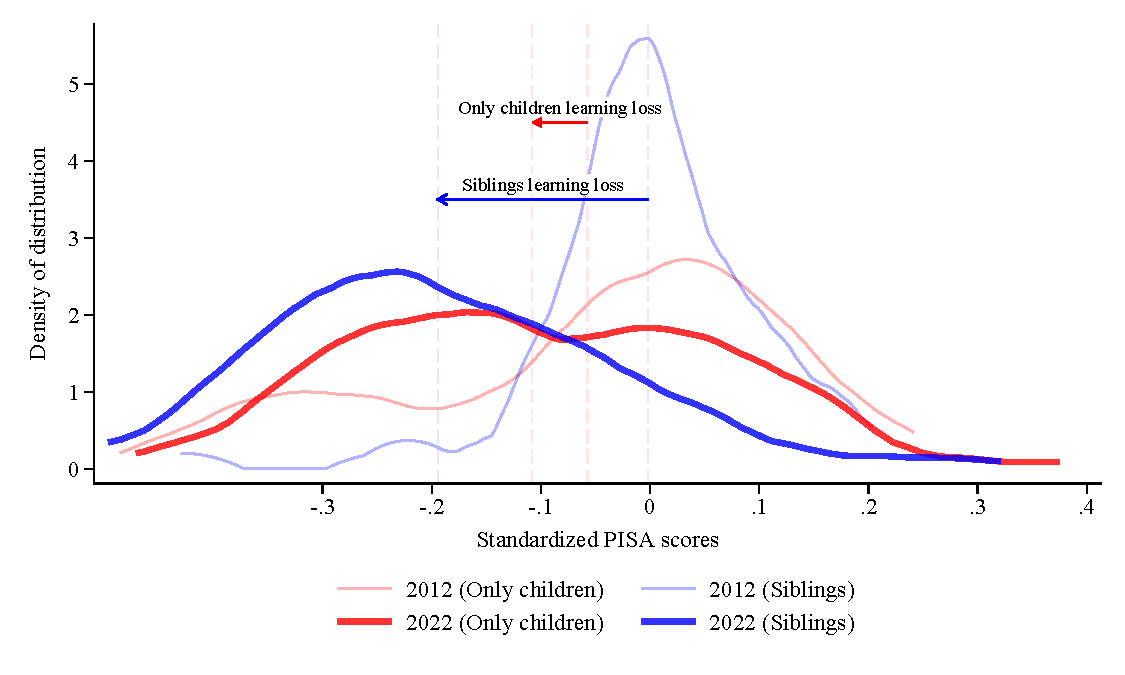
\includegraphics[width=\textwidth]{./FIGURES/Descriptive/PISA_distribution_2012_2022_PV4MATH.pdf}
        \caption{Learning gaps in Mathematics by year}
        \label{fig:1a}
    \end{subfigure}
    
    \vspace{1em} % Add some vertical space between subfigures
    
    \begin{subfigure}{\textwidth}
        \centering
        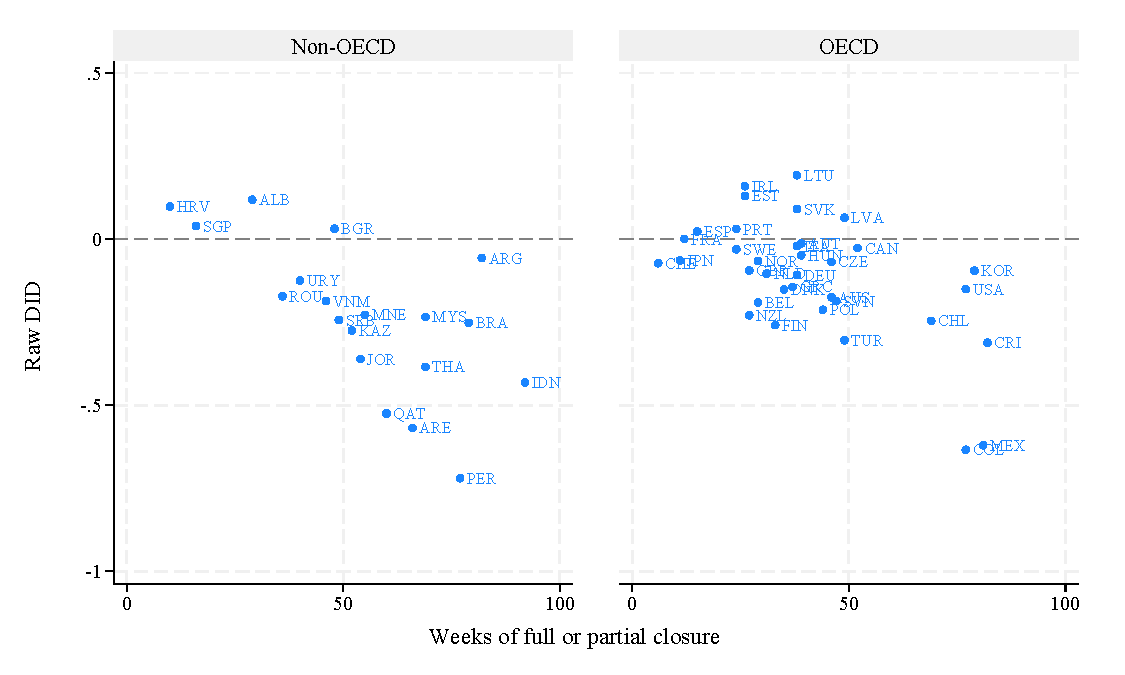
\includegraphics[width=\textwidth]{./FIGURES/Descriptive/PISA_raw_DID_PV4MATH_not_fully_open.pdf}
        \caption{Change in learning gaps by duration of school closure for OECD and Non-OECD countries.}
        \label{fig:1b}
    \end{subfigure}
    
    \caption{Learning gaps around the world}
    \label{fig:pisa}
\end{figure}



\begin{figure}[htbp]
    \centering
    
    \begin{subfigure}{\textwidth}
        \centering
        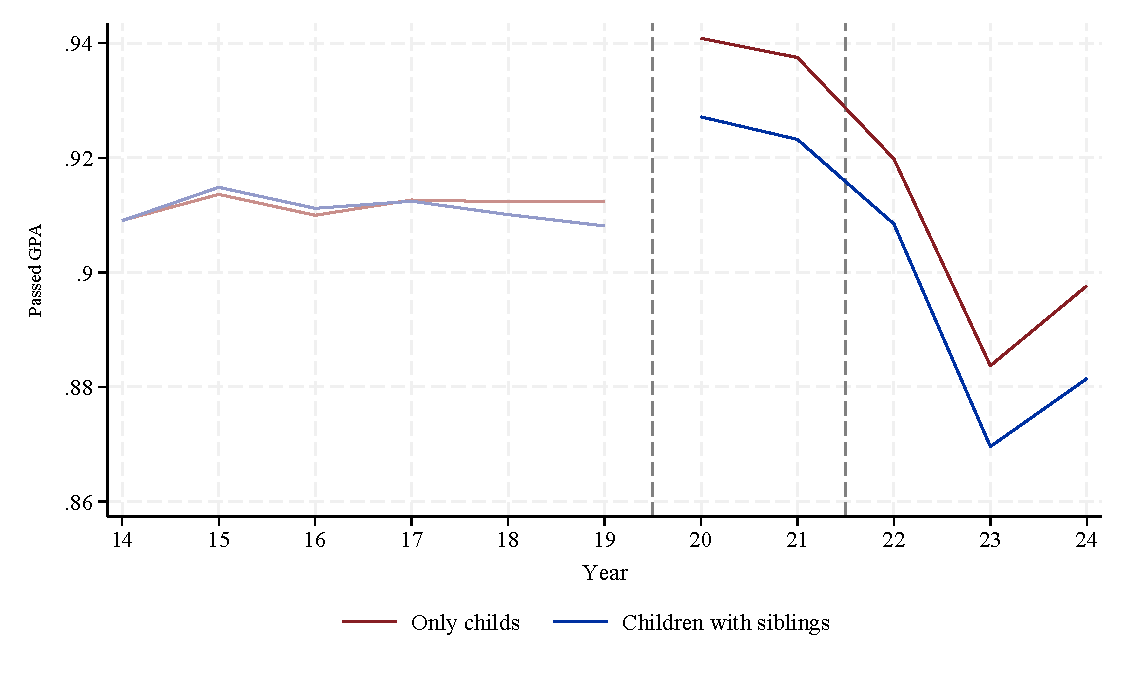
\includegraphics[width=\textwidth]{./FIGURES/Descriptive/raw_total_elm_pass_math_siblings.pdf}
        \caption{\% of students with a A in Mathematics from 1st-6th grade}
        \label{fig:trend_pass}
    \end{subfigure}
    
    \vspace{1em} % Add some vertical space between subfigures
    
    \begin{subfigure}{\textwidth}
        \centering
        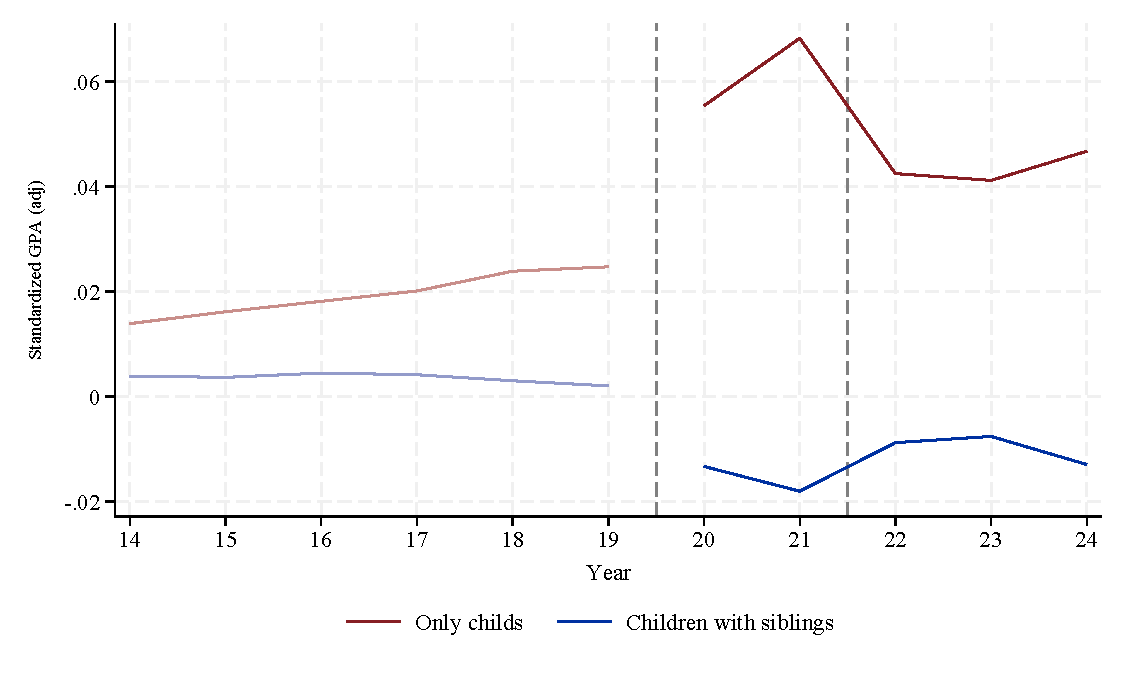
\includegraphics[width=\textwidth]{./FIGURES/Descriptive/raw_total_elm_std_gpa_m_adj_siblings.pdf}
        \caption{Average GPA standardized within school-grade-year from 1st-6th grade}
        \label{fig:trend_gpa}
    \end{subfigure}
    
    \caption{Trends in education outcomes for only children and children with siblings}
    \label{fig:trend}
\end{figure}


\begin{figure}[htbp]
    \centering
    
    \begin{subfigure}{\textwidth}
        \centering
        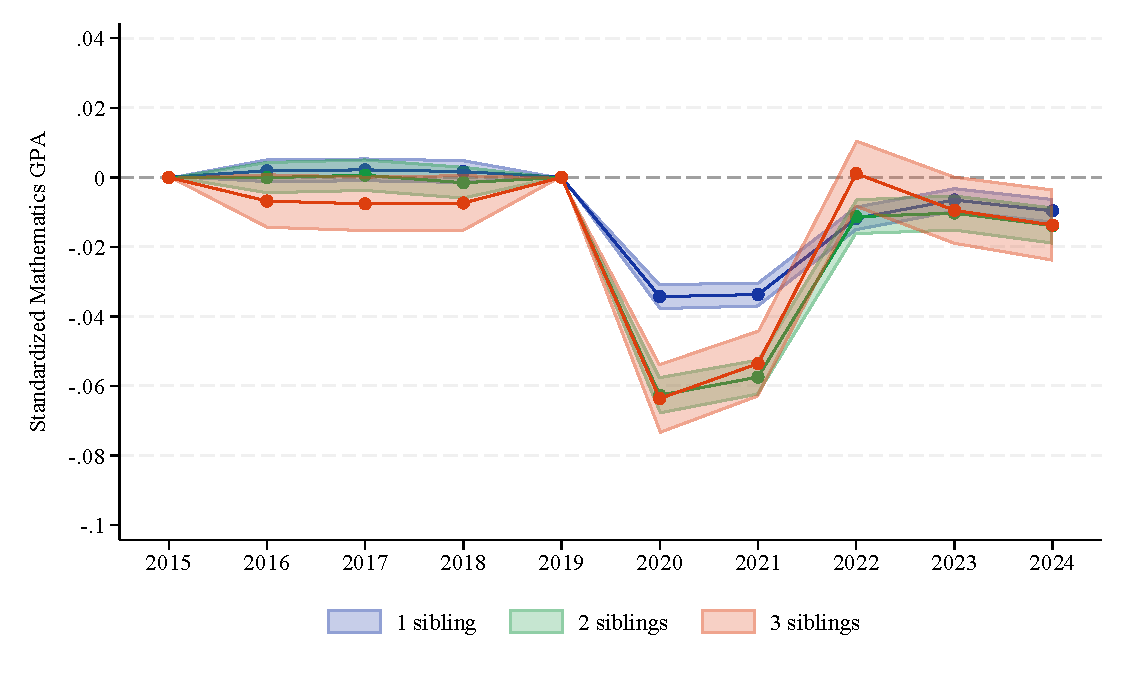
\includegraphics[width=\textwidth]{./FIGURES/Event Study/covid_event_bysibs_all_all_std_gpa_m_adj_Tsiblings_Soldest_4.pdf}
        \caption{Event Study}
        \label{fig:main_result_event}
    \end{subfigure}
    
    \vspace{1em} % Add some vertical space between subfigures
    
    \begin{subfigure}{\textwidth}
        \centering
        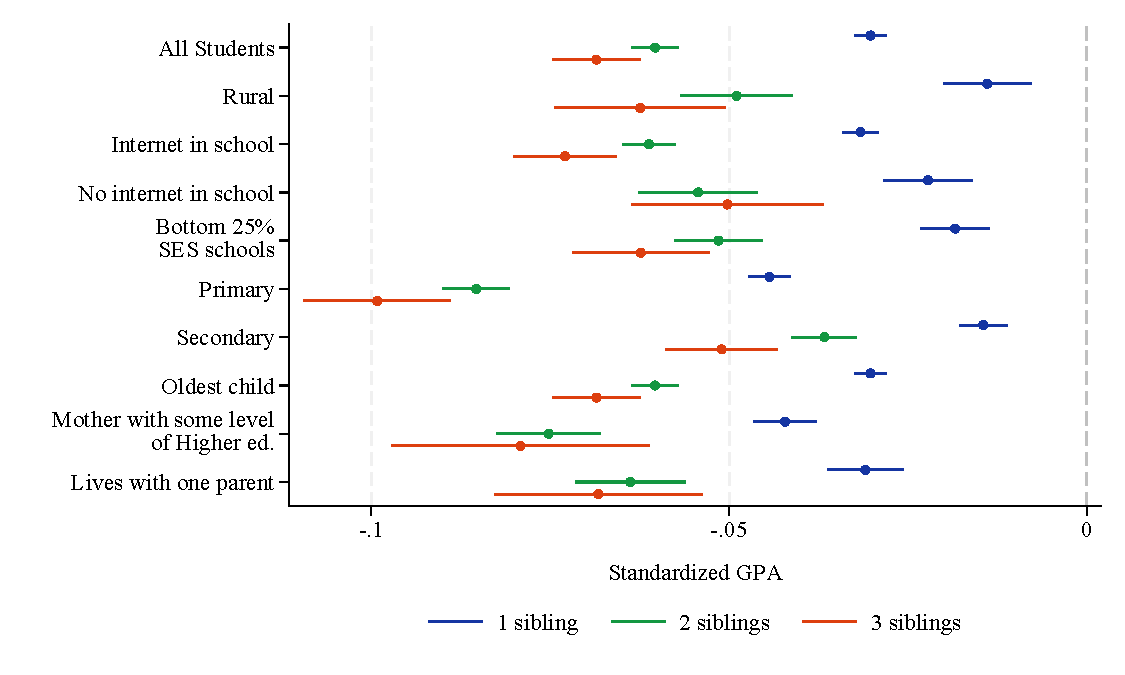
\includegraphics[width=\textwidth]{./FIGURES/TWFE/covid_twfe_summ_bysibs_all_20-21_gpa_m_adj_Tsiblings_Soldest_4.pdf}
        \caption{Change in gap between children with siblings and only childs}
        \label{fig:main_result_twfe}
    \end{subfigure}
    
    \caption{Learning gap between only childs and siblings}
    \label{fig:main_result}
\end{figure}


\clearpage

%RD-first grade
\makeatletter
\@ifclassloaded{beamer}{%
       \centering
       \resizebox{0.6\textwidth}{!}%
}{%
       \begin{table}[!tbp]\centering\def\sym#1{\ifmmode^{#1}\else\(^{#1}\)\fi}
       \centering
       \caption{TWFE on 8th grade GPA and standardized exams controlling for baseline 2nd grade standardized exams}
       \label{tab:twfe_ece}
       \resizebox{0.95\textwidth}{!}%
}
{
\makeatother
\begin{tabular}{lcccc}
\toprule
\cmidrule(lr){2-5}
& \multicolumn{4}{c}{TWFE} \\
\cmidrule(lr){2-5}
& 1-3 siblings & 1 sibling & 2 siblings & 3 siblings  \\
\cmidrule(lr){2-2} \cmidrule(lr){3-3} \cmidrule(lr){4-4} \cmidrule(lr){5-5}
& (1) & (2) & (3) & (4) \\
\bottomrule
&  &  & &  \\
&  &  & &  \\
\multicolumn{5}{l}{Panel A: GPA } \\
Mathematics         &      -0.099***&      -0.011   &      -0.036***&      -0.059***\\
                    &     (0.009)   &     (0.009)   &     (0.011)   &     (0.015)   \\
                    &               &               &               &               \\
Observations        &     326,669   &     279,833   &     225,092   &     179,575   \\
 
&  &  & &  \\
Reading             &      -0.099***&      -0.010   &      -0.031***&      -0.034** \\
                    &     (0.009)   &     (0.009)   &     (0.010)   &     (0.015)   \\
                    &               &               &               &               \\
Observations        &     326,669   &     280,846   &     225,840   &     180,218   \\
 
&  &  & &  \\
\multicolumn{5}{l}{Panel B: Standardized Exams } \\
Mathematics         &      -0.034***&      -0.017** &      -0.044***&      -0.071***\\
                    &     (0.006)   &     (0.007)   &     (0.008)   &     (0.011)   \\
                    &               &               &               &               \\
Observations        &     409,527   &     282,640   &     227,403   &     181,370   \\
 
&  &  & &  \\
Reading             &      -0.013** &       0.002   &      -0.022***&      -0.046***\\
                    &     (0.006)   &     (0.006)   &     (0.008)   &     (0.011)   \\
                    &               &               &               &               \\
Observations        &     409,690   &     282,769   &     227,486   &     181,466   \\
 

\bottomrule
\end{tabular}
}
\@ifclassloaded{beamer}{%
}{%
       \end{table}
}

\makeatletter
\@ifclassloaded{beamer}{%
       \centering
       \resizebox{0.6\textwidth}{!}%
}{%
       \begin{table}[!tbp]\centering\def\sym#1{\ifmmode^{#1}\else\(^{#1}\)\fi}
       \centering
       \caption{TWFE on GPA by baseline resources}
       \label{tab:twfe_gpa_baseline_survey_1_pairall}
       \resizebox{0.65\textwidth}{!}%
}
{
\makeatother
\begin{tabular}{lccc}
\toprule
\cmidrule(lr){2-4}
& \multicolumn{3}{c}{TWFE} \\
\cmidrule(lr){2-4}
& 1 sibling & 2 siblings & 3 siblings  \\
\cmidrule(lr){2-2} \cmidrule(lr){3-3} \cmidrule(lr){4-4}
& (1) & (2) & (3)\\
\bottomrule
&  &  &  \\
&  &  &   \\
\multicolumn{4}{l}{\textit{Panel A: All studentes}} \\
\hspace{3mm}Mathematics&      -0.028***&      -0.061***&      -0.080***\\
                    &     (0.004)   &     (0.005)   &     (0.009)   \\
 
%&  &  &   \\
\hspace{3mm}Reading &      -0.018***&      -0.044***&      -0.052***\\
                    &     (0.004)   &     (0.005)   &     (0.009)   \\
                    &               &               &               \\
\hspace{3mm}Observations&   1,285,073   &   1,038,874   &     906,608   \\
 
&  &  &   \\
\multicolumn{4}{l}{\textit{Panel B: Low SES Households (Q1)}} \\
\hspace{3mm}Mathematics&      -0.009   &      -0.028***&      -0.061***\\
                    &     (0.007)   &     (0.009)   &     (0.014)   \\
 
%&  &  &   \\
\hspace{3mm}Reading &      -0.003   &      -0.016*  &      -0.040***\\
                    &     (0.007)   &     (0.009)   &     (0.014)   \\
                    &               &               &               \\
\hspace{3mm}Observations&     312,464   &     264,200   &     226,444   \\
 
&  &  &   \\
\multicolumn{4}{l}{\textit{Panel C: High SES Households (Q4)}} \\
\hspace{3mm}Mathematics&      -0.037***&      -0.065***&      -0.113***\\
                    &     (0.008)   &     (0.014)   &     (0.034)   \\
 
%&  &  &   \\
\hspace{3mm}Reading &      -0.029***&      -0.070***&      -0.017   \\
                    &     (0.008)   &     (0.014)   &     (0.034)   \\
                    &               &               &               \\
\hspace{3mm}Observations&     257,212   &     199,735   &     179,355   \\
 
&  &  &   \\
\multicolumn{4}{l}{\textit{Panel D: Households with no PC or Internet}} \\
\hspace{3mm}Mathematics&      -0.032***&      -0.079***&      -0.067***\\
                    &     (0.006)   &     (0.009)   &     (0.019)   \\
 
%&  &  &   \\
\hspace{3mm}Reading &      -0.023***&      -0.056***&      -0.051***\\
                    &     (0.006)   &     (0.009)   &     (0.019)   \\
                    &               &               &               \\
\hspace{3mm}Observations&     454,966   &     366,342   &     320,367   \\
 
&  &  &   \\
\multicolumn{4}{l}{\textit{Panel E: Households with both PC and Internet}} \\
\hspace{3mm}Mathematics&      -0.023***&      -0.035***&      -0.098***\\
                    &     (0.006)   &     (0.009)   &     (0.015)   \\
 
%&  &  &   \\
\hspace{3mm}Reading &      -0.008   &      -0.039***&      -0.061***\\
                    &     (0.006)   &     (0.009)   &     (0.015)   \\
                    &               &               &               \\
\hspace{3mm}Observations&     438,221   &     355,035   &     307,508   \\
 

\bottomrule
\end{tabular}
}
\@ifclassloaded{beamer}{%
}{%
       \end{table}
}

\makeatletter
\@ifclassloaded{beamer}{%
       \centering
       \resizebox{0.6\textwidth}{!}%
}{%
       \begin{table}[!tbp]\centering\def\sym#1{\ifmmode^{#1}\else\(^{#1}\)\fi}
       \centering
       \caption{WFE on GPA by baseline achievement and expectations}
       \label{tab:twfe_gpa_baseline_survey_2_pairall}
       \resizebox{0.65\textwidth}{!}%
}
{
\makeatother
\begin{tabular}{lccc}
\toprule
\cmidrule(lr){2-4}
& \multicolumn{3}{c}{TWFE} \\
\cmidrule(lr){2-4}
& 1 sibling & 2 siblings & 3 siblings  \\
\cmidrule(lr){2-2} \cmidrule(lr){3-3} \cmidrule(lr){4-4}
& (1) & (2) & (3)\\
\bottomrule
&  &  &  \\
&  &  &   \\
\multicolumn{4}{l}{\textit{Panel A: All studentes}} \\
\hspace{3mm}Mathematics&      -0.028***&      -0.061***&      -0.080***\\
                    &     (0.004)   &     (0.005)   &     (0.009)   \\
 
%&  &  &   \\
\hspace{3mm}Reading &      -0.018***&      -0.044***&      -0.052***\\
                    &     (0.004)   &     (0.005)   &     (0.009)   \\
                    &               &               &               \\
\hspace{3mm}Observations&   1,285,073   &   1,038,874   &     906,608   \\
 
&  &  &   \\
\multicolumn{4}{l}{\textit{Panel B: Student in bottom quartile of achievement}} \\
\hspace{3mm}Mathematics&       0.001   &      -0.042***&      -0.106***\\
                    &     (0.007)   &     (0.010)   &     (0.015)   \\
 
%&  &  &   \\
\hspace{3mm}Reading &       0.009   &      -0.036***&      -0.064***\\
                    &     (0.008)   &     (0.010)   &     (0.016)   \\
                    &               &               &               \\
\hspace{3mm}Observations&     261,349   &     220,666   &     193,655   \\
 
&  &  &   \\
\multicolumn{4}{l}{\textit{Panel C: Student in top quartile of achievement}} \\
\hspace{3mm}Mathematics&      -0.045***&      -0.101***&      -0.140***\\
                    &     (0.007)   &     (0.011)   &     (0.023)   \\
 
%&  &  &   \\
\hspace{3mm}Reading &      -0.032***&      -0.069***&      -0.090***\\
                    &     (0.007)   &     (0.011)   &     (0.023)   \\
                    &               &               &               \\
\hspace{3mm}Observations&     364,927   &     282,401   &     245,220   \\
 
&  &  &   \\
\multicolumn{4}{l}{\textit{Panel D: Max Expectation: Finish school}} \\
\hspace{3mm}Mathematics&      -0.003   &      -0.030   &      -0.054*  \\
                    &     (0.014)   &     (0.019)   &     (0.030)   \\
 
%&  &  &   \\
\hspace{3mm}Reading &      -0.027*  &      -0.031   &      -0.059*  \\
                    &     (0.015)   &     (0.019)   &     (0.031)   \\
                    &               &               &               \\
\hspace{3mm}Observations&      84,652   &      71,387   &      61,974   \\
 
&  &  &   \\
\multicolumn{4}{l}{\textit{Panel E: Max Expectation: 4-year college or grad school}} \\
\hspace{3mm}Mathematics&      -0.033***&      -0.067***&      -0.095***\\
                    &     (0.004)   &     (0.006)   &     (0.011)   \\
 
%&  &  &   \\
\hspace{3mm}Reading &      -0.022***&      -0.049***&      -0.073***\\
                    &     (0.004)   &     (0.006)   &     (0.011)   \\
                    &               &               &               \\
\hspace{3mm}Observations&   1,039,027   &     830,658   &     724,846   \\
 

\bottomrule
\end{tabular}
}
\@ifclassloaded{beamer}{%
}{%
       \end{table}
}



\clearpage
\makeatletter
\@ifclassloaded{beamer}{%
       \centering
       \resizebox{0.6\textwidth}{!}%
}{%
       \begin{table}[!tbp]\centering\def\sym#1{\ifmmode^{#1}\else\(^{#1}\)\fi}
       \centering
       \caption{Effects of younger sibling delaying school on older sibling standardized exams - 1 - m - a -  - 365}
       \label{tab:rd_summ_1_m_a_365}
       \resizebox{0.95\textwidth}{!}%
}
{
\makeatother
\resizebox{\textwidth}{!}{
\begin{tabular}{lccc}
\toprule
\cmidrule(lr){2-4}
& \multicolumn{3}{c}{Standardized GPA} \\
\cmidrule(lr){2-4}
& Pre-Covid & Covid & Post-Covid  \\
& 2018-2019 & 2020-2021 & 2022-2023  \\
\cmidrule(lr){2-2} \cmidrule(lr){3-3} \cmidrule(lr){4-4}
& (1) & (2) & (3)  \\
\bottomrule
&  &  &   \\
\multirow{2}{*}{\shortstack[l]{Younger sibling born after \\ school-entry cutoff}}&      -0.023***&      -0.001   &      -0.023***\\
                    &     (0.007)   &     (0.007)   &     (0.006)   \\
Local Linear        &         Yes   &         Yes   &         Yes   \\
                    &               &               &               \\
Observations        &     358,861   &     354,044   &     447,536   \\
Counterfactual mean &       0.058   &       0.020   &       0.050   \\
Bandwidth           &         365   &         365   &         365   \\
 

\bottomrule
\end{tabular}
}
\@ifclassloaded{beamer}{%
}{%
       \end{table}
}

\makeatletter
\@ifclassloaded{beamer}{%
       \centering
       \resizebox{0.6\textwidth}{!}%
}{%
       \begin{table}[!tbp]\centering\def\sym#1{\ifmmode^{#1}\else\(^{#1}\)\fi}
       \centering
       \caption{Effects of younger sibling delaying school on older sibling standardized exams and parental investment}
       \label{tab:rd_ece_index_365}
       \resizebox{0.95\textwidth}{!}%
}
{
\makeatother
\begin{tabular}{lccccc}
\toprule
& \multicolumn{2}{c}{Pre-Covid}  & \multicolumn{3}{c}{Post-Covid} \\
& \multicolumn{2}{c}{2018-2019}  & \multicolumn{3}{c}{2022-2024}  \\
\cmidrule(lr){2-3} \cmidrule(lr){4-6}
& Mathematics & Reading & Mathematics & Reading & Parental Investment  \\
& (1) & (2) & (3) & (4) & (5) \\
\bottomrule
&  &  &  & &  \\
\multirow{2}{*}{\shortstack[l]{Younger sibling born after \\ school-entry cutoff}}&      -0.025*  &      -0.023*  &      -0.009   &      -0.012   &      -0.035***\\
                    &     (0.014)   &     (0.012)   &     (0.013)   &     (0.010)   &     (0.013)   \\
Local Linear        &         Yes   &         Yes   &         Yes   &         Yes   &         Yes   \\
                    &               &               &               &               &               \\
Observations        &      86,605   &      86,602   &     104,983   &     105,064   &     101,766   \\
Counterfactual mean &      -0.105   &      -0.083   &       0.194   &       0.288   &      -0.004   \\
Bandwidth           &         365   &         365   &         365   &         365   &         365   \\
 

\bottomrule
\end{tabular}
}
\@ifclassloaded{beamer}{%
}{%
       \end{table}
}









\end{document}